\IfFileExists{IEEEtran.cls}{
  \documentclass[conference]{IEEEtran}
  \newcommand{\ieeeavailable}{1}
}{
  \documentclass[10pt,twocolumn]{article}
  \usepackage[a4paper,top=18mm,bottom=20mm,left=16mm,right=16mm,columnsep=6mm]{geometry}
  \newenvironment{IEEEkeywords}{\par\small\noindent\textbf{Index Terms---}}{\par}
}

\usepackage[T1]{fontenc}
\usepackage[utf8]{inputenc}
\usepackage[expansion=false]{microtype}
\usepackage{graphicx}
\usepackage{booktabs}
\usepackage{array}
\usepackage{amsmath}
\usepackage{url}
\usepackage{xcolor}
\usepackage{tikz}
\usetikzlibrary{arrows.meta,positioning,fit}
\usepackage[hidelinks]{hyperref}

\title{Uchko: A Hybrid XGBoost and Bayesian Knowledge Tracing Platform for Adaptive Mathematics Practice}

\author{
\ifdefined\ieeeavailable
\IEEEauthorblockN{Tarik Agi\'{c} and Azra Kuri\'{c}}
\IEEEauthorblockA{Faculty of Electrical Engineering, University of Sarajevo\\
Sarajevo, Bosnia and Herzegovina\\
\{tagic2, akuric1\}@etf.unsa.ba}
\else
Tarik Agi\'{c} and Azra Kuri\'{c}\\
\small Faculty of Electrical Engineering, University of Sarajevo\\
\small Sarajevo, Bosnia and Herzegovina\\
\small \{tagic2, akuric1\}@etf.unsa.ba
\fi
}

\date{}

\begin{document}
\maketitle

\begin{abstract}
Adaptive learning systems must connect predictive models with persistent learner state, curriculum-aligned content, and a usable delivery interface. This paper presents Uchko, a deployable web platform for adaptive middle-school mathematics practice. The system combines two complementary models trained on FoundationalASSIST data: an XGBoost classifier estimates the probability that a learner will independently solve a candidate problem, while Bayesian Knowledge Tracing (BKT) maintains an interpretable mastery probability for each skill. A deterministic selection policy first considers a learner's weakest skills and then favors problems whose predicted success probability is near a 0.65 target. To reduce target leakage and improve generalization to unseen learners, all sequential features use only prior interactions and train, validation, and test partitions are disjoint at the student level. After filtering and metadata joins, the modeling data contain 1,693,947 interactions from 5,000 students. XGBoost achieves 0.8122 ROC AUC, 0.7440 accuracy, and 0.5061 log loss on the held-out test students, compared with 0.6929 ROC AUC and 0.6075 log loss for a history baseline. BKT obtains 0.6850 ROC AUC and remains valuable as a transparent online state estimator. The models are integrated into a Django application with role-based student and professor views, persistent attempts and sessions, curriculum exploration, sanitized imported content, and explicit separation between answer correctness and unaided success. The result demonstrates how a compact hybrid architecture can turn offline educational data mining models into an end-to-end adaptive learning experiment.
\end{abstract}

\begin{IEEEkeywords}
adaptive learning, educational data mining, knowledge tracing, XGBoost, student modeling, intelligent tutoring systems
\end{IEEEkeywords}

\section{Introduction}
Students working through the same curriculum differ in prior knowledge, pace, and need for support. Adaptive learning attempts to address this variation by estimating learner state and selecting an appropriate next activity. The technical challenge is broader than predicting whether an answer will be correct: a useful platform must preserve student histories, represent curricular skills, provide actionable information to teachers, and convert model outputs into stable pedagogical decisions. Recent reviews therefore describe adaptive learning as a system-level problem spanning student modeling, content, sequencing, feedback, and governance \cite{kabudi2021adaptive,tan2025platforms}.

Knowledge tracing is central to this problem. Classical BKT models skill mastery as a latent variable updated after each observation \cite{corbett1994knowledge}. Deep Knowledge Tracing (DKT) later demonstrated that recurrent networks can learn richer representations directly from interaction sequences \cite{piech2015dkt}. However, greater predictive capacity does not by itself determine how a system should choose content, communicate progress, or handle assisted answers. Interpretable state estimates and reliable software behavior remain particularly important in educational deployments.

This paper presents Uchko, an end-to-end adaptive mathematics platform created as an implementation and experimental demonstration. It builds on FoundationalASSIST, a recent dataset containing complete question content, student responses, curriculum alignment, and approximately 1.7 million interactions from 5,000 learners \cite{worden2026foundationalassist}. Uchko uses the protected interaction log only for offline model training; the application imports problem and skill metadata but does not distribute the interaction records.

The principal contributions are:
\begin{itemize}
    \item a leakage-aware student-success model evaluated on entirely unseen learners;
    \item a hybrid design in which XGBoost ranks candidate difficulty while skill-specific BKT provides an interpretable, continuously updated mastery state;
    \item a concrete adaptive policy that targets productive challenge and avoids immediately repeating recently shown items;
    \item a persistent, role-aware Django implementation that exposes learning activities to students and aggregate progress to their professor; and
    \item a deliberate distinction between literal answer correctness and independent success, preventing hints or revealed answers from being counted as unaided evidence of mastery.
\end{itemize}

The goal is not to claim improved learning outcomes from an offline experiment. Rather, the work evaluates next-response prediction and demonstrates how the resulting models can be integrated responsibly into a usable adaptive workflow.

\subsection{Related Work}
Research on adaptive educational systems spans intelligent tutoring, learning analytics, and educational data mining. Systematic reviews find substantial technical activity but fewer evaluations that connect model improvements to learners' real challenges and classroom deployment \cite{kabudi2021adaptive,tan2025platforms}. ASSISTments is a particularly relevant foundation because it combines online mathematics practice with immediate feedback and teacher-facing information; a randomized evaluation reported improved student achievement from online mathematics homework using the platform \cite{rochelle2016assistments}. Uchko does not attempt to reproduce that causal claim. It uses a newer ASSISTments-derived dataset to evaluate prediction and to implement a deployable adaptation loop.

Within knowledge tracing, BKT remains influential because its parameters have explicit cognitive interpretations, while DKT and later attentive models capture richer dependencies in student sequences \cite{corbett1994knowledge,piech2015dkt,ghosh2020akt}. Surveys emphasize that comparisons are sensitive to preprocessing, splitting, and model configuration \cite{abdelrahman2023survey}. Uchko therefore prioritizes a reproducible, student-disjoint evaluation and uses deep sequence modeling only as a proposed controlled extension. The distinctive focus of this work is not a novel knowledge-tracing architecture, but the integration of complementary prediction and mastery components into a tested application whose instructional policy is inspectable.

\section{Background and Design Rationale}
\subsection{Complementary Student Models}
BKT represents each skill through four parameters: initial mastery $P(L_0)$, learning $P(T)$, guessing $P(G)$, and slipping $P(S)$. Given the current mastery $P(L)$, the probability of a correct response is
\begin{equation}
P(C)=P(L)(1-P(S))+(1-P(L))P(G).
\end{equation}
After observing a response, Bayes' rule updates mastery, followed by a learning transition. BKT is compact and pedagogically legible, but its conditional independence assumptions restrict the interactions it can represent.

Gradient-boosted trees provide a complementary capability. XGBoost constructs an additive ensemble of regularized decision trees and is designed for scalable learning from sparse, heterogeneous features \cite{chen2016xgboost}. It can use item identifiers, problem metadata, and non-linear interactions among prior-performance variables without assuming a single latent state. In Uchko, XGBoost predicts near-term success while BKT answers a different question: how the system's belief about a particular skill should change after new evidence.

The hybrid choice also supports graceful failure. If a problem identifier was not observed during fitting, the preprocessing pipeline ignores the unseen one-hot category while retaining history and metadata features. If a skill lacks sufficient evidence for a stable BKT fit, a global parameter set is used. These fallbacks are important for an application whose curriculum may evolve.

\subsection{From Prediction to Selection}
Purely maximizing predicted correctness would repeatedly offer easy items. Conversely, always choosing the lowest-mastery skill may produce problems that are too difficult. Uchko uses a bounded heuristic inspired by the idea of maintaining productive challenge. Among candidates attached to the eight weakest available skills, the system evaluates up to five items per skill. For candidate item $i$, it minimizes
\begin{equation}
s_i=\left|\hat{p}_i-0.65\right|+0.10m_i,
\end{equation}
where $\hat{p}_i$ is the XGBoost success probability and $m_i$ is current BKT mastery. The first term strongly prefers a predicted success rate near 65\%; the smaller second term breaks close decisions in favor of weaker skills. The twenty most recently attempted items are initially excluded, with a fallback if this removes every valid candidate. The 0.65 target is a transparent design parameter rather than a learned claim about optimal pedagogy.

\section{Data and Methodology}
\subsection{Dataset and Responsible Use}
FoundationalASSIST contains mathematics interactions aligned with Common Core standards and retains richer question and response information than conventional identifier-only knowledge-tracing benchmarks \cite{worden2026foundationalassist}. The raw release reports 3,395 problems and about 1.7 million interactions. Uchko's training pipeline loads interaction identifiers, problem identifiers, hint use, answer-reveal indicators, binary scores, timestamps, and anonymized user identifiers. It joins these records to problem and skill metadata.

Rows with missing timestamps or non-binary scores are removed, interaction identifiers are deduplicated, and problems with ambiguous duplicate metadata records are excluded before a validated many-to-one join. The resulting dataset has 1,693,947 interactions from 5,000 students. The Django content importer produces 3,353 learning items, of which 2,483 have a supported, usable numeric or single-choice answer for adaptive practice. The curriculum view exposes 164 imported skills.

The interaction file is access-controlled data. It was processed only in the university environment, was not committed to the repository, and is not loaded into the deployed application database. Only trained artifacts, aggregate metrics, problem content, and skill metadata are used by the application. This separation reduces unnecessary exposure of historical student records.

\subsection{Leakage-Aware Preprocessing}
Interactions are ordered by student, timestamp, and interaction identifier. Every historical feature is computed strictly before the current target. The model uses five categorical variables---problem, problem set, problem type, answer type, and primary skill---and thirteen numerical variables. Numerical features include problem part, number of attached skills, prior user attempts and successes, Laplace-smoothed user accuracy, accumulated hints and answer reveals, previous correctness, previous hint use, capped time since the previous interaction, and analogous skill-specific counts and smoothed accuracy.

For example, the smoothed user accuracy before interaction $t$ is
\begin{equation}
a_t=\frac{c_{<t}+1}{n_{<t}+2},
\end{equation}
where $c_{<t}$ and $n_{<t}$ include only earlier responses. This avoids undefined cold-start values and shrinks small histories toward 0.5.

Students, rather than rows, are shuffled with seed 42 and divided 70/15/15. The training partition contains 1,185,585 rows from 3,500 students; validation contains 253,894 rows from 750 students; and test contains 254,468 rows from 750 students. Student-disjoint evaluation is stricter than a random row split because the model cannot exploit the same learner identity across training and test data.

Categorical variables are one-hot encoded with rare levels grouped below a frequency of twenty. Numeric values are median-imputed and scaled without centering to preserve sparse matrices. The preprocessing object is fitted only on the training partition and serialized with the final feature schema.

\subsection{Models and Evaluation}
Three success-prediction references were constructed. A global baseline assigns the training-set success prevalence to every case. A history baseline uses the student's smoothed prior accuracy. A linear logistic model, implemented with stochastic gradient descent, provides a validation-stage learned baseline. The selected XGBoost classifier uses a binary logistic objective, learning rate 0.05, maximum depth 8, row and column subsampling of 0.85, and up to 1,000 trees. Early stopping with patience 30 is performed only against validation log loss; the test partition is evaluated once after selection.

BKT parameters are fitted by bounded maximum likelihood. A global parameter vector is learned from all training sequences. A skill receives its own parameters only when the training data contain at least 1,000 interactions from at least 50 students; otherwise, the global vector is recorded as a fallback. This produces 95 skill-specific fits and 57 fallback entries. BKT predictions are generated sequentially, resetting state at student boundaries.

Evaluation reports threshold-independent ROC AUC together with accuracy and F1 at a 0.5 threshold. Because the adaptive policy consumes probabilities, log loss and Brier score are also reported. These proper scoring rules penalize poorly calibrated confidence rather than assessing ranking alone \cite{brier1950verification}.

\begin{figure*}[t]
\centering
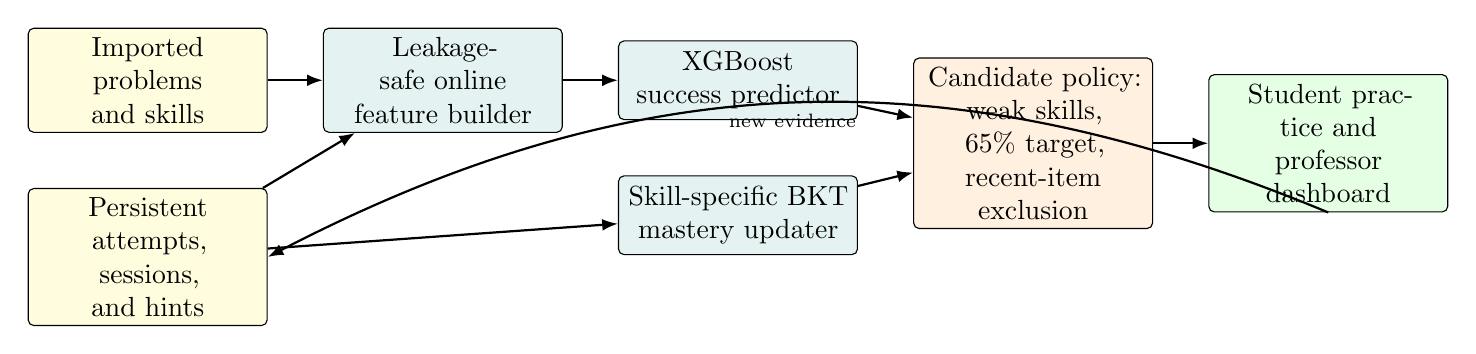
\begin{tikzpicture}[
node distance=7mm and 7mm,
box/.style={draw, rounded corners=2pt, align=center, minimum height=10mm, text width=28mm, fill=blue!4},
model/.style={box, fill=teal!10},
data/.style={box, fill=yellow!13},
arr/.style={-{Latex[length=2mm]}, thick}
]
\node[data] (content) {Imported problems\\and skills};
\node[data, below=of content] (history) {Persistent attempts,\\sessions, and hints};
\node[model, right=of content] (features) {Leakage-safe online\\feature builder};
\node[model, right=of features] (xgb) {XGBoost\\success predictor};
\node[model, below=of xgb] (bkt) {Skill-specific BKT\\mastery updater};
\node[box, right=of xgb, yshift=-8mm, fill=orange!12] (policy) {Candidate policy:\\weak skills, 65\% target,\\recent-item exclusion};
\node[box, right=of policy, fill=green!10] (ui) {Student practice and\\professor dashboard};
\draw[arr] (content) -- (features);
\draw[arr] (history) -- (features);
\draw[arr] (features) -- (xgb);
\draw[arr] (history) -- (bkt);
\draw[arr] (xgb) -- (policy);
\draw[arr] (bkt) -- (policy);
\draw[arr] (policy) -- (ui);
\draw[arr, bend right=25] (ui.south) to node[below, font=\scriptsize]{new evidence} (history.east);
\end{tikzpicture}
\caption{Uchko's hybrid adaptive loop. XGBoost predicts candidate success, BKT tracks skill mastery, and a deterministic policy converts both outputs into the next practice activity.}
\label{fig:architecture}
\end{figure*}

\section{System Implementation}
Figure~\ref{fig:architecture} summarizes the implemented loop. Uchko is a server-rendered Django application backed by a relational database. The data model includes users with student or professor roles, courses, enrollments, knowledge components, learning items, learning sessions, attempts, and per-enrollment knowledge states. Database transactions and row locking protect mastery and attempt updates from inconsistent concurrent writes.

At inference time, the application reconstructs the same features used during training from a student's persisted history. The serialized preprocessor and XGBoost model run on CPU even though model fitting used GPU acceleration. Candidate items must have a supported answer and belong to an active course. After submission, answer checking supports tolerance-aware numeric responses and single-choice alternatives.

A critical implementation detail is the separation of \emph{answer correctness} from \emph{independent success}. If the final submitted answer is correct after a hint or after revealing the answer, the interface acknowledges correctness, but the attempt is not treated as independent mastery evidence. BKT is updated using
\begin{equation}
y^{\mathrm{ind}}=y^{\mathrm{answer}}\land(h=0)\land\neg r,
\end{equation}
where $h$ is the hint count and $r$ indicates that the answer was revealed. This choice aligns the online signal with the training target's treatment of assistance and prevents a student from inflating mastery simply by requesting the answer. The interface explicitly explains why mastery may decrease after a correct but assisted response.

The student experience includes a role-aware home page, adaptive practice, progress summaries, curriculum exploration, and account information. Professors can inspect enrolled students and skill-level progress without accessing another course's records. Imported question bodies and options can contain HTML and MathML, so they are sanitized through explicit tag, attribute, CSS-property, URL-scheme, and image-host allowlists before rendering. Automated tests cover authorization, content sanitization, repeated-question scoring, and the adaptive workflow; continuous integration runs framework checks, migration checks, dependency checks, and the complete test suite.

\begin{figure*}[t]
\centering
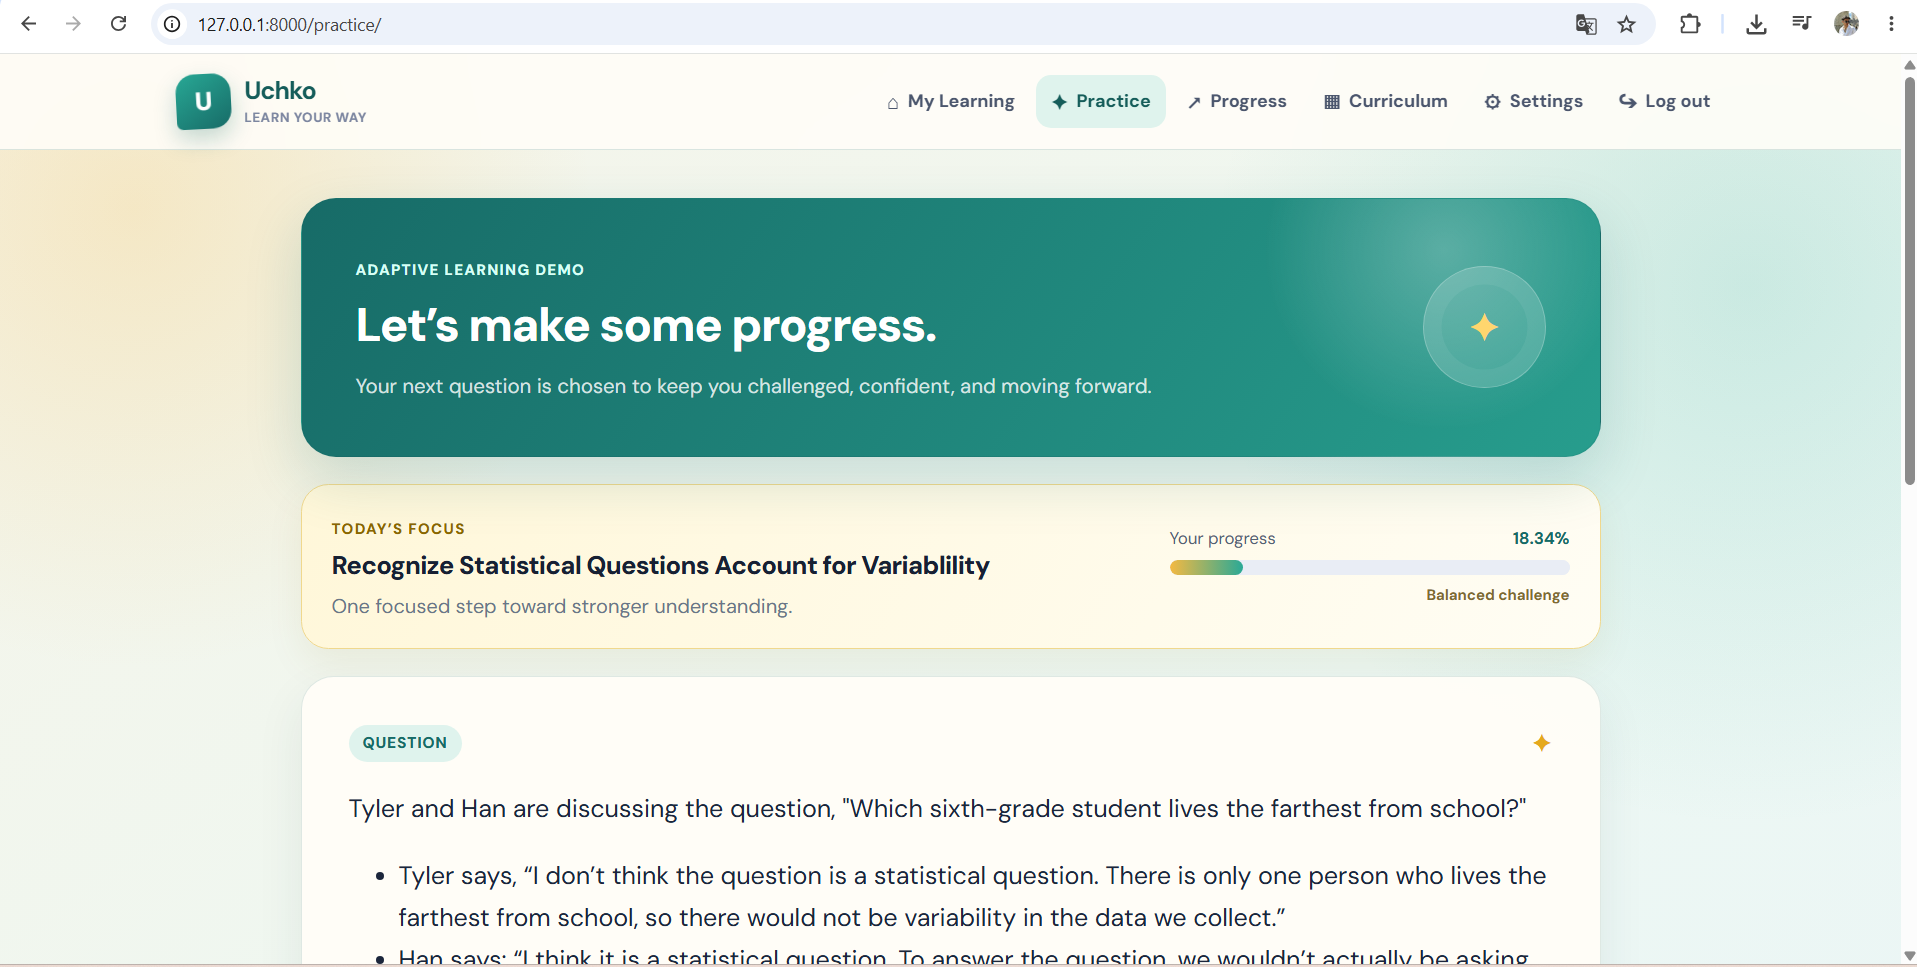
\includegraphics[width=0.88\textwidth]{figures/uchko_practice.png}
\caption{The implemented student practice interface exposes the selected skill and progress while keeping model-specific diagnostics outside the primary learning task.}
\label{fig:interface}
\end{figure*}

\section{Results}
Table~\ref{tab:results} reports held-out student performance. The global validation baseline has an AUC of 0.5 by construction and is omitted from the table for compactness. The linear model reaches 0.7868 AUC and 0.5393 log loss on validation, while validation results for XGBoost are 0.8087 and 0.5113, respectively. This validation advantage motivated selection of XGBoost before final testing.

\begin{table}[t]
\centering
\caption{Performance on 750 held-out test students}
\label{tab:results}
\setlength{\tabcolsep}{3.3pt}
\begin{tabular}{lccccc}
\toprule
Model & AUC & Acc. & F1 & Log loss & Brier \\
\midrule
History & 0.6929 & 0.6728 & 0.7601 & 0.6075 & 0.2098 \\
BKT & 0.6850 & 0.6772 & 0.7671 & 0.6105 & 0.2106 \\
XGBoost & \textbf{0.8122} & \textbf{0.7440} & \textbf{0.8057} & \textbf{0.5061} & \textbf{0.1693} \\
\bottomrule
\end{tabular}
\end{table}

XGBoost improves AUC by 0.1193 over the history baseline and reduces log loss by approximately 16.7\%. Its Brier score is lower by approximately 19.3\%, indicating that the gain is not limited to thresholded classification. Similar validation and test metrics---0.8087 versus 0.8122 AUC and 0.5113 versus 0.5061 log loss---provide no sign of a large validation-to-test collapse.

BKT does not outperform the history baseline in AUC or probabilistic loss, although its accuracy and F1 are slightly higher at the chosen threshold. This result should not be hidden: under the present feature and split definitions, BKT is not the strongest next-response predictor. Its contribution is instead an interpretable state transition that can be updated after every response and inspected per skill. The hybrid system assigns prediction and state estimation to the models that best support each role.

The evaluation also illustrates why accuracy alone is insufficient. The training success prevalence is 0.6141, so an always-positive tendency can produce a superficially substantial F1 score. ROC AUC and proper probability losses more clearly distinguish the models. For the adaptive policy, probability quality is especially relevant because candidate ranking depends directly on distance from the 0.65 target.

\section{Discussion}
The experiment supports three conclusions. First, prior learner history and problem metadata together contain considerably more predictive information than aggregate history alone. XGBoost benefits from non-linear interactions among sparse item categories, temporal signals, hint histories, and skill-specific performance. Second, student-disjoint partitions offer evidence that the model generalizes to new learner accounts rather than memorizing students seen during training. Third, deploying prediction requires additional design decisions that offline metrics do not resolve. The target probability, recent-item exclusion window, weakest-skill set size, and handling of assistance are transparent policy choices and should eventually be validated through user studies.

The study has limitations. FoundationalASSIST reflects one platform, mathematics curriculum, and historical logging policy. Offline next-response accuracy is not evidence of improved learning, retention, motivation, or fairness. The current split tests unseen students but does not simulate chronological dataset drift. XGBoost can express complex feature interactions, yet individual predictions are less pedagogically transparent than BKT states. The 0.65 success target is a reasonable design heuristic, not an experimentally optimized value. Finally, only numeric and single-choice items with recoverable answers are presently used in practice, reducing content coverage from 3,353 imported items to 2,483 usable items.

A deep sequential model is a natural extension, but it should be evaluated as an experiment rather than assumed to be superior. A compact DKT model can encode each skill-response pair and use a gated recurrent network to predict the next response \cite{piech2015dkt}. For a fair comparison, it must use the same student split, prior-only sequences, target definition, and probability metrics. If it materially improves log loss or AUC, its added complexity must still be weighed against inference cost, cold-start behavior, and interpretability. If it does not improve performance, the negative result would strengthen the case for the current compact hybrid design.

\section{Conclusion}
Uchko demonstrates an end-to-end path from protected educational interaction data to adaptive web-based practice. On unseen students, XGBoost substantially outperforms an aggregate-history baseline for next-response prediction, while BKT provides a simple and inspectable per-skill state. A deterministic policy combines both signals to focus on weak skills at a controlled level of challenge. Persistent data models, role-based authorization, safe content rendering, and explicit treatment of assisted answers turn the model experiment into a functioning platform rather than an isolated notebook. The remaining research question is educational impact: future work should test whether the policy improves learning and whether its recommendations remain fair, understandable, and useful in authentic classrooms.

\ifdefined\ieeeavailable
\bibliographystyle{IEEEtran}
\else
\bibliographystyle{unsrt}
\fi
\bibliography{references}

\end{document}
